%----------------------------------------------------------------------------------------
%	PACKAGES AND THEMES
%----------------------------------------------------------------------------------------
\PassOptionsToPackage{table}{xcolor}
\documentclass[aspectratio=169,xcolor=dvipsnames,11pt]{beamer}
\usetheme{SimplePlusAIC}
\usepackage{amsmath}
\usepackage{animate}
\usepackage{hyperref}
\usepackage{cleveref}
\usepackage{caption}
\usepackage{graphicx} % Allows including images
%\usepackage{subfig}
\usepackage{subcaption}
\usepackage{booktabs} % Allows the use of \toprule, \midrule and  \bottomrule in tables
\usepackage{svg} %allows using svg figures
\usepackage{tikz}
\usepackage{makecell}
\usepackage{multirow}
\usepackage{appendixnumberbeamer}
\usepackage{wrapfig}
\usepackage{verbatim}
\usepackage{tcolorbox}
%\usepackage[dvipsnames]{xcolor}

\usepackage{hhline}
\usepackage{relsize}
\usepackage{bm}
%Select the Epilogue font (requires luaLatex or XeLaTex compilers)
%\setsansfont{Epilogue}[
  %  Path=./epilogueFont/,
  %  Scale=0.9,
  %  Extension = .ttf,
   % UprightFont=*-Regular,
   % BoldFont=*-Bold,
   % ItalicFont=*-Italic,
    %BoldItalicFont=*-BoldItalic
    %]
    \usefonttheme[onlymath]{serif}
% \usepackage{ eulervm } % Euler VM as math serif font

\newcommand*{\defeq}{\stackrel{\text{def}}{=}}
\newcommand{\grad}{\nabla}
\newcommand{\lap}{\Delta}
\newcommand{\weaklyto}{\rightharpoonup}
\newcommand{\weakstar}{\stackrel{*}\rightharpoonup}
\newcommand{\cts}{\hookrightarrow}
\newcommand{\ctsDense}{\xhookrightarrow{d}}
\newcommand{\ctsCompact}{\xhookrightarrow{c}}
\newcommand{\E}{\mathbb{E}}
\newcommand{\pP}{\mathbb{P}}
\newcommand{\R}{\mathbb{R}}
\newcommand{\ER}{\overline{\mathbb{R}}}
\newcommand{\cR}{\mathcal{R}}
\newcommand{\cJ}{\mathcal{J}}
\newcommand{\cG}{\mathcal{G}}
\newcommand{\CVaR}{\textup{CVaR}}
\newcommand{\D}{\textup{ d}}
\newcommand{\dd}{\mathrm{d}}
\newcommand{\fa}{\text{for all }}
\DeclareMathOperator*{\essinf}{\vphantom{p}ess\,inf}
\DeclareMathOperator{\sigmoid}{expit} % a.k.a. logistic sigmoid

\usepackage[ruled,vlined,algo2e]{algorithm2e}
\crefname{algocf}{algorithm}{algorithms}
 \usepackage{caption}

\usepackage{tcolorbox}  % For fancy boxes
\usepackage{lipsum}     % For dummy text

% Define a custom style for the box
\tcbuselibrary{skins, breakable}
\newtcolorbox[auto counter, number within=section]{roundedshadowbox}[2][]{
    colback=white, % Background color (kept white)
    colframe=black, % Border color
    boxrule=0.5pt, % Border thickness
    arc=5mm, % Rounded corners
    shadow=true, % Drop shadow effect
    width=\linewidth, % Full width box
    title=#2, % Title text
    #1 % Additional options (e.g., width override)
}

\usepackage{pgfplots}
\pgfplotsset{compat=1.18}

%\PassOptionsToPackage{table}{xcolor}
%\documentclass[aspectratio=169,xcolor=dvipsnames,11pt]{beamer}
%\usetheme{SimplePlusAIC}
%\usepackage{amsmath}
%\usepackage{hyperref}
%\usepackage{cleveref}
%\usepackage{caption}
%\usepackage{graphicx} % Allows including images
%\usepackage{subcaption}
%\usepackage{booktabs} % Allows the use of \toprule, \midrule and  \bottomrule in tables
%\usepackage{svg} %allows using svg figures
%\usepackage{tikz}
%
%\usepackage{pgfplots}
%\pgfplotsset{compat=1.18}
%
%\usepackage{makecell}
%\usepackage{multirow}
%\usepackage{appendixnumberbeamer}
%\usepackage{wrapfig}
%\usepackage{verbatim}
%\usepackage{tcolorbox}
%\usepackage{hhline}
%\usepackage{relsize}
%\usepackage{bm}
%
%\usefonttheme[onlymath]{serif}
%    
\newcommand{\C}{\mathbb C}

%
%%\font\nullfont=cmr10
%
%\usepackage{tcolorbox}  % For fancy boxes
%\usepackage{lipsum}     % For dummy text
%
%% Define a custom style for the box
%\tcbuselibrary{skins, breakable}
%\newtcolorbox[auto counter, number within=section]{roundedshadowbox}[2][]{
%    colback=white, % Background color (kept white)
%    colframe=black, % Border color
%    boxrule=0.5pt, % Border thickness
%    arc=5mm, % Rounded corners
%    shadow=true, % Drop shadow effect
%    width=\linewidth, % Full width box
%    title=#2, % Title text
%    #1 % Additional options (e.g., width override)
%}


%----------------------------------------------------------------------------------------
%	TITLE PAGE
%----------------------------------------------------------------------------------------

\title[\quad\quad\quad LVPP Course II]{The Latent Variable Proximal Point Method II: Derivation, Analysis, and First Numerical Experiments
 } % The short title appears at the bottom of every slide, the full title is only on the title page
%\subtitle{Subtitle}

\author{\small{\bf Thomas M. Surowiec}}

\institute[T.M. Surowiec]{Department of Numerical Analysis and Scientific Computing \newline Simula Research Laboratory \newline Oslo, Norway}
% Your institution as it will appear on the bottom of every slide, maybe shorthand to save space


\date[EMS School]{ {\footnotesize 
K\'acov, Czechia, 15-20 June 2025}}
%----------------------------------------------------------------------------------------
%	PRESENTATION SLIDES
%----------------------------------------------------------------------------------------

\begin{document}

\begin{frame}[plain]
%\setbeamertemplate{footline}{}
\titlepage
\end{frame}

\begin{frame}{Overview}
\tableofcontents
\end{frame}

\section{Penalty and Approximation Methods}
 \begin{frame}\frametitle{Frame Title}
    \begin{enumerate}
    	\item Quadratic Penalty
		\begin{enumerate}
			\item Definition
			\item Connection to Moreau-Yosida regularization
			\item Asymptotic convergence
			\item Advantages/Disadvantages
			\item Path-following
		\end{enumerate}
	\item Barrier Penalty
		\begin{enumerate}
			\item Definition
			\item Outer vs. Inner approximation
			\item Primal-dual formulation
			\item PD does not force $u$ to be nonnegative, this has to be done with careful line search
		\end{enumerate}
	\item Augmented Lagrangian (Ito, Kunisch 1990)
		\begin{enumerate}
			\item Definition
			\item A dual-adaptive quadratic penalty scheme, roots in proximal point (Rockafellar)
			\item For computation, we need $\lambda$ to have a pointwise interpretation, but this may not be guaranteed
			\item This forces $r \to +\infty$ (as opposed to finite dimensions)
		\end{enumerate}
    \end{enumerate}
 \end{frame}
 
 \begin{frame}\frametitle{A Mathematical Fruitfly} 
  \begin{beamercolorbox}[rounded=true, shadow=true, wd=\textwidth]{block title}\centering
  In order to make a nuanced comparison between several methods, we introduce each method using the obstacle problem.
  The methods themselves are widely applicable.
  \end{beamercolorbox}\hfill
  
\visible<2->{
\begin{minipage}{0.7\linewidth}
\begin{beamercolorbox}[rounded=true, shadow=true, wd=\textwidth]{block body}
 We seek a minimizer $u$ of the objective functional:
 \begin{equation*}
 	J(v)
 	=
 	\frac{1}{2}
 	\int_\Omega |\nabla v|^2 \dd x
 	-
 	\int_\Omega f v\dd x
 	\,,
 \end{equation*}
 over
 \[
 K = \{ v \in H^1_0(\Omega) \mid  v \ge \varphi \text{~a.e. }  \}.
 \] 
 Here, $f \in L^2(\Omega)$ and  $\varphi \in H^1(\Omega)$, $\varphi|_{\Gamma} \le 0$.
\end{beamercolorbox}
\end{minipage}%
\begin{minipage}{0.3\linewidth}
 \centering
\begin{figure}
	\centering
	\begin{tikzpicture}
		\node at (-4.2,1.2) {\scriptsize 
	    	$u$};
		\node at (-3.35,0) {\includegraphics[height=1.25in]{../Part I/figures/obstacle_new.png}};
		\node at (-2.2,-1.35) {\scriptsize 
	    	$\varphi$};
    \end{tikzpicture}
\end{figure}
\end{minipage}}
 \end{frame}
 
 \begin{frame}\frametitle{Penalty Methods}
   \begin{beamercolorbox}[rounded=true, shadow=true, wd=\textwidth]{block body}
This approach involves relaxing the constraints with a smooth penalty function $\beta : K \to \mathbb R$, where $\beta$ is usually convex, $C^{1,1}$ and ideally satisfies
\[
\beta(u) = 0 \text{ if } u \in K\quad \text{ and }\quad \beta(u) > 0 \text{ otherwise. }
\]
  \end{beamercolorbox}
%\begin{minipage}{\textwidth}
% \centering 
 \begin{figure}
% \resizebox{0.3\textwidth}{0.25\textwidth}{%
  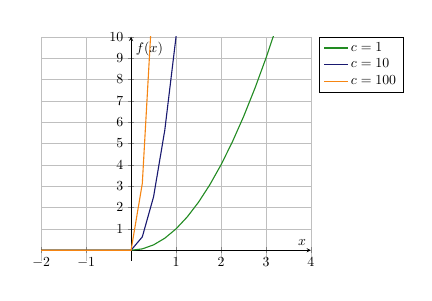
\begin{tikzpicture}[scale=0.5]
    \begin{axis}[
        axis lines=middle, % Draw axes through the origin
        xlabel=$x$,
        ylabel=$f(x)$,
        xmin=-2, xmax=4, % Adjust x-range as needed
        ymin=-0.5, ymax=10, % Adjust y-range as needed
        grid=both, % Add a grid
        grid style={line width=.1pt, draw=gray!10}, % Style the grid lines
        major grid style={line width=.2pt,draw=gray!50}, % Style major grid lines
        xtick distance=1, % Tick marks every 1 unit on x-axis
        ytick distance=1, % Tick marks every 1 unit on y-axis
        % Add a legend
        legend pos=outer north east, % Position the legend
        legend cell align=left,
        no markers, % Don't put markers on the plots
    ]

    % Define the function with a placeholder for c
    % We use 'max(0,x)^2' for the (x)^2 part, and then multiply by c
    % PGFPlots works with degrees, so we need to be careful with functions that are not trigonometric.
    % max(0, x) is directly supported.

    % Plot for c = 0.5
    \addplot[domain=-2:4, ForestGreen, thick] {1 * max(0,x)^2};
    \addlegendentry{$c=1$};

    % Plot for c = 1
    \addplot[domain=-2:4, MidnightBlue, thick] {10.0 * max(0,x)^2};
    \addlegendentry{$c=10$};

    % Plot for c = 2
    \addplot[domain=-2:4, BurntOrange, thick] {50.0 * max(0,x)^2};
    \addlegendentry{$c=100$};

    \end{axis}
\end{tikzpicture}
%}
\caption{Plot of the typical quadratic penalty function used for inequality constraints $f_c(x) = c\max\{0,x\}^2$.}
  \label{fig:tikz-example}
\end{figure}
%\end{minipage}
 \end{frame}

\section{The Proximal Point Method}
 \begin{frame}\frametitle{Frame Title}
    \begin{enumerate}
    	\item Martinet, Rockafellar
	\item Bregman, Nemirovskij Yudin
	\item Convergence statements
    \end{enumerate}
 \end{frame}

\section{Derivation of the Latent Variable Proximal Point Method}
 \begin{frame}\frametitle{Frame Title}
        \begin{enumerate}
    	\item Formal application to the obstacle problem
	\item Failure of the primal version
	\item Invention of the latent variable
	\item Discretization approaches
    \end{enumerate}
 \end{frame}
 
 
 \section{First Numerical Experiments}
 \begin{frame}\frametitle{Frame Title}
        \begin{enumerate}
    	\item
    \end{enumerate}
 \end{frame}
 
  \section{Theoretical Results}
 \begin{frame}\frametitle{Frame Title}
        \begin{enumerate}
    	\item
    \end{enumerate}
 \end{frame}


\end{document}